\chapter{Implementierung}
Für diese Arbeit wurde der \acl{SSB} sowohl in PostgreSQL als auch in einer angepassten Form in Redis durchgeführt.
\section{\acl{SSB} in PostgreSQL}
\subsection{Generierung der \acs{SSB}-Daten}
% Hier ganze Anleitung im Anhang verlinken
Es ist möglich, die Daten für den \acl{SSB} mit dem Programm ssb-dbgen~\cite{phillips_electrumssb-dbgen_2023} zu generieren.
Mit diesem Programm können verschiedene Datenskalierungen erzeugt werden.
Hierbei werden .tbl-Dateien generiert, die in eine SQL-basierte Datenbank importiert werden können.
\subsection{Ausführen des \acl{SSB} in PostgreSQL}

% Zeiten anpassen
Es existiert ein GitHub-Repository ~\cite{nukoyokohama_ssb-postgres_2023}, das eine Anleitung und Skripte für das Ausführen des \ac{SSB} in PostgreSQL bereitstellt.
Zur Ausführung wurde ein Docker-Container mit dem Image "postgres-standard" erstellt.
Dabei wurden die Standardwerte der PostgreSQL-Konfiguration verwendet.
Anschließend wurden die .tbl-Dateien und Skripte des Repositories in diesen Container geladen. % Deutschen Begriff für gebinded finden
Nach der Erstellung des Containers wird zunächst das Skript 'tables.sql' ausgeführt, um die Tabellen in der Datenbank anzulegen.
Danach können die Daten in die Tabellen importiert werden, indem das Skript 'load.sql' ausgeführt wird.
Abschließend kann der Benchmark durch die Ausführung des Skripts 'explain-analyze.sql' aus dem Repository durchgeführt werden.
% Hier ganze Anleitung im Anhang verlinken

% TODO: Ansatz aus Paper beleuchten
\section{\acs{SSB} in Redis}
Im Gegensatz zu relationalen Datenbanken ist das Konzept der Tabelle in Redis unbekannt.
Daten können daher nicht auf verschiedene Tabellen verteilt werden.
Es ist möglich, mehrere Datenbanken in Redis zu verwenden. Viele Erweiterungen bieten jedoch nur Unterstützung für die erste Datenbank.
Die Verwendung von mehreren Datenbanken in Redis wird als Anti-Pattern betrachtet und ist daher nicht empfohlen~\cite{prickett_answer_2022}.
Stattdessen werden künstliche Namensräume eingeführt, indem Präfixe zu Schlüsseln hinzugefügt werden.
Die Daten können damit in Kategorien eingeteilt werden.
Jede Zeile der .tbl-Dateien entspricht einer Zeile in einer der SQL-Tabellen.
Jede Zeile wurde unter einem einzigartigen Schlüssel mit dem Datentyp HASH in Redis gespeichert.

Im Rahmen dieser Forschung wurden verschiedene Ansätze zur Speicherung von Daten in Redis gewählt.

\subsection{Wahl des Datentyps in Redis}
Von den gängigen Datentypen in Redis unterstützen nur Hashes, JSON und Sorted Sets eine Key-Value-Struktur. Theoretisch können Daten auch in Strings gespeichert werden und durch die Volltextsuche von Redisearch ist es auch möglich nach Daten zu suchen, jedoch ist dies wesentlich komplizierter als bei Hashes und JSON.
In Sorted Sets können nur begrenzte numerische Werte gespeichert werden was sie für die SSB-Daten nicht nutzbar macht, da dort unter anderem auch Texte gespeichert werden müssen.
Hashes und JSON bieten beide die Möglichkeit, beliebige Daten in einer Key-Value-Struktur zu speichern und dann mir RediSearch auch nach diesen Daten zu suchen.
Hashes benötigen dafür jedoch erheblich weniger Speicherplatz als JSON.
JSON wird in einer deserialisierten Form gespeichert und benötigt etwas Overhead zusätzlich zu den eigentlichen Daten~\cite{redis_json-ram-usage_nodate}.
Hashes sind dagegen optimiert um Speicher zu sparen~\cite{redis_memory-optimization_nodate}.
Mit dem Befehl \emph{MEMORY USAGE} kann der Speicherverbrauch eines Elements in Redis angezeigt werden~\cite{redis_memory-usage-command-redis_nodate}.

% Dafür sorgen dass Abbildung an richitger Stelle ist...
% Abbildung statt Figure bei \Cref
In \Cref{pic:redis-hash-vs-json-memory} wird der Vergleich der Speicherplatznutzung dargestellt, wobei dieselben Informationen einmal in Form eines Hash und einmal in Form von JSON gespeichert sind. In diesem Beispiel belegt das JSON-Format 694 Byte, während das Hash-Format nur 288 Byte benötigt, was einer Reduzierung um 58,5\% entspricht.
\begin{figure}[!h]  % force the figure to be placed here
    \centering
    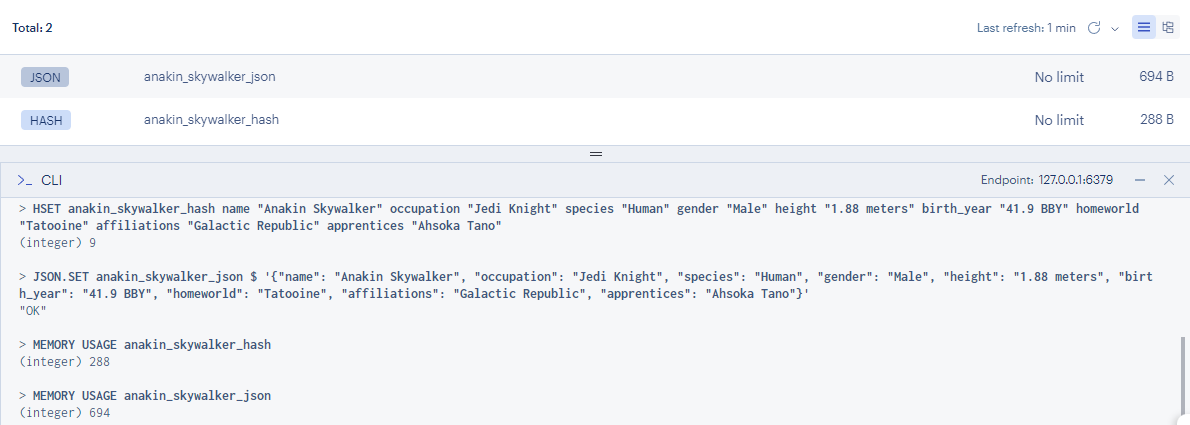
\includegraphics[width=1\textwidth]{pictures/redis/redis_hash_vs_json_memory.png}
    \caption{Vergleich des Speicherplatznutzung zwischen HASH und JSON}
    \label{pic:redis-hash-vs-json-memory}
\end{figure}


\subsection{RediSearch für Abfragen}
% Beschreiben, warum Redisearch zwingend notwendig ist

% Ab hier alles mit deepl write überarbeiten

\subsection{Speichern der Daten in Pseudotabellen}
In diesem Ansatz werden die Daten nach den Tabellen kategorisiert.
Die Schlüssel der Einträge bestehen dabei aus einer Kombination des Tabellennamens und der ursprünglichen Primärschlüssel (siehe \cref{code:ssb-redis-structur-example}).

\begin{lstlisting}[
    language=java,
    caption=Aufbau der Schlüssel der \ac{SSB}-Daten in Redis,
    label=code:ssb-redis-structur-example
]
date:19931104
\end{lstlisting}

\subsubsection{Einfügen der Daten mit einem Scala-Programm}
% TODO: Auf digitalen Anhang verweisen
Um die Daten in Redis einzufügen, wurde ein Scala-Programm geschrieben.
Zunächst liest das Programm die .tbl-Dateien ein und erstellt für jede Zeile ein Array aus Strings, wobei die Strings die Werte der einzelnen Spalten repräsentieren.
Anschließend werden diese Arrays unter Verwendung des generierten Schlüssels in Redis eingefügt.
Da die LINEORDER-Tabelle einen zusammengesetzten Primärschlüssel verwendet, besteht auch der Schlüssel in Redis aus den Werten zweier Felder.
Dabei wird der Befehl HSET verwendet, der das Speichern eines Arrays als HASH in Redis ermöglicht.

\begin{lstlisting}[
    language=scala,
    float,
    caption=Einfügen der Daten in Pseudotabellen in Redis,
    label=code:ssb-redis-insert-pseudotables-snippet
]
// This method processes several lines in one go in order to use the redis pipeline,
// hence it receives a Sequence of lines as input
def insertIntoRedis(
    data: Seq[String],
    databaseName: String,
    dataStructure: Array[String],
    isLineOrder: Boolean,
    pipeline: Pipeline
): Unit = {
  data.foreach { line =>
    val values = line.split("\\|") // Splitting the pipe-separated lines
    val valueIterator = values.iterator
    dataStructure.foreach { key =>
      // Check if key needs to consist of one or two primary keys
      if (valueIterator.hasNext) {
        if (isLineOrder) {
          pipeline.hset(
            (databaseName + ":" + values(0) + ":" + values(1)).getBytes,
            key.getBytes,
            valueIterator.next().getBytes()
          )
        } else {
          pipeline.hset(
            (databaseName + ":" + values(0)).getBytes,
            key.getBytes,
            valueIterator.next().getBytes()
          )
        }
      }
    }
  }
  pipeline.sync()
}


\end{lstlisting}
% Darauf achten, dass Listing an richtiger Stelle ist
% TODO: Redis Pipeline in Grundlagen erklären und hie rverlinken

\subsubsection{Denormalisierter Ansatz}
Der Ansatz mit der tabellarischen Struktur erfordert das Verbinden von Pseudotabellen (Joins).
Es sind mehrere Abfragen erforderlich, um die Daten entweder clientseitig oder über ein LUA-Skript filtern zu können.
Dieser Umstand macht diesen Ansatz ineffizient und es ist unmöglich, die Berechnungen vollständig auf Seiten der Datenbank auszuführen.

Im Gegensatz zum tabellarischen Ansatz steht der denormalisierte Ansatz.

Um Joins vollständig zu vermeiden und eine vollständige clientseitige Verarbeitung zu ermöglichen, werden die Daten vollständig denormalisiert.
Die Tabellen werden aufgelöst
und alle Dimensionstabellen (DATE, PART, SUPPLIER, CUSTOMER) in die Faktentabelle (LINEORDER) integriert.

\subsubsection{Denormalisieren der Daten und Einfügen in Redis}
Um die Daten zu denormalisieren und in Redis zu speichern, wurde das Scala-Programm angepasst.

Das Programm definiert eigene Datentypen für die Daten der verschiedenen Tabellen (ShortenedLineorderObject, ShortenedCustomerObject, ShortenedSupplierObject, ShortenedPartObject, ShortenedDateObject).
Diese Datentypen enthalten Strings für alle Spalten der ursprünglichen Tabellen, die in den \acs{SSB}-Queries verwendet werden.
Des Weiteren wird im Zuge der Implementierung ein neuer Datentyp namens "DenormalizedObject" definiert,
der die Attribute anderer Datentypen in sich vereint und somit die denormalisierten Daten enthält.

Das Programm liest zunächst alle .tbl-Dateien ein, erzeugt daraus Objekte mit den zuvor definierten Datentypen und speichert diese als Werte in einer Map ab. Als Schlüssel dient dabei der Primärschlüssel in Form eines Strings.

Anschließend erfolgt eine Iteration über sämtliche "LINEORDER"-Einträge.
Für jedes Fremdschlüssel-Attribut wird das zugehörige Objekt aus der entsprechenden Map abgerufen.
Wenn also ein ShortenedLineorderObject beispielsweise den Wert X für suppkey hat, wird das ShortenedSupplierObject mit dem Schlüssel X aus der ShortenedSupplierObject-Map geladen.

Sobald alle Fremdschlüssel aufgelöst sind, wird ein DenormalizedObject erstellt und zusammen mit den Primärschlüsseln des ShortenedLineorderObject als Schlüssel in Redis gespeichert. (siehe \cref{code:ssb-redis-insert-denormalized-snippet}).


\begin{lstlisting}[
    language=scala,
    float,
    caption=Einfügen der denormalisierten Daten in Redis (Auszug),
    label=code:ssb-redis-insert-denormalized-snippet
]
private def createDenormalizedMap(
    customerMap: Map[String, ShortenedCustomerObject],
    supplierMap: Map[String, ShortenedSupplierObject],
    partMap: Map[String, ShortenedPartObject],
    lineorderMap: Map[String, ShortenedLineorderObject],
    dateMap: Map[String, ShortenedDateObject]
): Unit = {

  lineorderMap.foreach { case (key, lineorder) =>
    val customer = 
      customerMap.getOrElse(lineorder.lo_custkey, ShortenedCustomerObject("", "", "", ""))
    val supplier = 
      supplierMap.getOrElse(lineorder.lo_suppkey, ShortenedSupplierObject("", "", "", ""))
    val part = 
      partMap.getOrElse(lineorder.lo_partkey, ShortenedPartObject("", "", "", ""))
    val date = 
      dateMap.getOrElse(lineorder.lo_orderdate, ShortenedDateObject("", ""))

    val denormalized = DenormalizedObject(
      lineorder.lo_orderkey,
      ...
      customer.c_city,
      customer.c_nation,
      ...
    )

    denormalizedMap += (key -> denormalized)
  }
}

private def insertDenormalizedObjectsIntoRedis(pipeline: Pipeline): Unit = {
  denormalizedMap.values.grouped(1000).foreach { denormalizedObjects =>
    denormalizedObjects.foreach { denormalizedObject =>
      val hash = Map(
        "lo_orderkey" -> denormalizedObject.lo_orderkey,
        ...
        "c_city" -> denormalizedObject.c_city,
        "c_nation" -> denormalizedObject.c_nation,
        ...
      )

      pipeline.hmset("lineorder:" + denormalizedObject.lo_orderkey + ":" + denormalizedObject.lo_linenumber, hash.asJava)
      numOfInsertedRecords = numOfInsertedRecords + 1
    }
    pipeline.sync()
  }
}


\end{lstlisting}

% Darauf hinweisen, dass hier natürlich Daten verlorengehen, da nur für SSB Queries relevante Daten gespeichert werden

\subsubsection{Anpassen der Queries}
Mit RediSearch lassen sich die SQL-Queries des \acf{SSB} sehr gut für Redis anpassen.
\section{Praktische Implementierung}

\subsection{Scala}

\subsection{Scala mit Lua}

\section{Limitierungen der Implementierung}
